
\subsubsection{Type-Erasure}
Il design pattern \textit{Type-Erasure} è un pattern che permette di avere vero e proprio polimorfismo 
object-oriented ma esponendo un API senza puntatori ed eventualmente ottimizzata con \textit{copy on write}.

\begin{figure}[H]
    \centering
        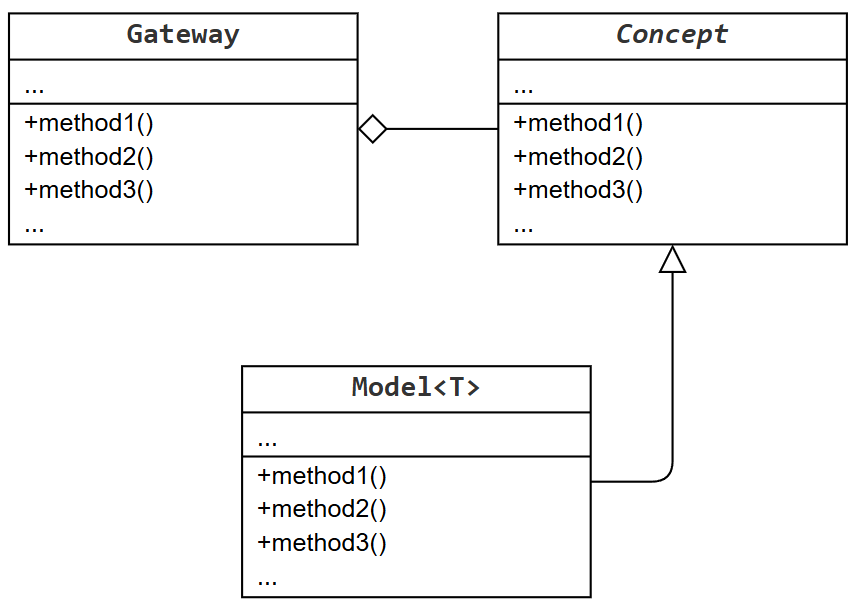
\includegraphics[width=0.7\textwidth]{../../Assets/TypeErasure.png}
    \caption{UML class diagram del pattern Type-Erasure}
\end{figure}

La classe \texttt{Gateway} è un esempio di implementazione di Type-Erasure. Essa viene utilizzata dai client 
come supertipo di tutti gli oggetti che implementano dei metodi pubblici chiamati \texttt{method1()}, 
\texttt{method2()},\texttt{method3()}, \texttt{method4()}, etc. \\

\newpage

Internamente essa possiede un puntatore a \texttt{Concept}, a cui è possibile assegnare 
puntatori ad oggetti di tipo \texttt{Model<T>} per ogni scelta di \texttt{T}. \\

A patto che \texttt{T} esponga la corretta API, la classe \texttt{Model<T>} può implementare i metodi chiamandoli 
direttamente su di un'istanza di \texttt{T} che essa possiede come membro interno. \\

Assegnare un oggetto di tipo \texttt{T} ad un \texttt{Gateway} è possibile grazie alla ridefinizione dell'operatore \texttt{=}
nella classe \texttt{Gateway}. Assegnando un oggetto di tipo \texttt{T} a un oggetto di tipo \texttt{Gateway} allora 
il suo puntatore a \texttt{Concept} sarà aggiornato per puntare all'indirizzo di memoria di una cella appositamente allocata 
per contenere un \texttt{Model<T>} costruito a partire dall'oggetto \texttt{T} ricevuto. \\

\vspace{0.5cm}
\begin{lstlisting}[language=C++, frame=single]
#define ABSTRACT 0
template <typename T>
class Concept {
    public:
        virtual void method1() = ABSTRACT;
        virtual void method2() = ABSTRACT;
        //...
};

template <typename T>
class Model : public Concept {
    private:
        T object;
    public:
        Model(T obj) : object(obj) {}
        void method1() override { object.method1(); }
        void method2() override { object.method2(); }
        //...
};

class Gateway {
    private:
        std::unique_ptr<Concept> concept = nullptr;

    public:
        template<typename T>
        Gateway& operator=(T obj) {
            concept = std::make_unique<Model<T>>(obj);
        }

        void method1() { concept->method1(); }
        void method2() { concept->method2(); }
        //...
}

\end{lstlisting}
\vspace{0.5cm}

\newpage

questo pattern consente di assegnare a oggetti di tipo \texttt{Gateway} oggetti di tipo \texttt{T} che implementano
l'API corretta, e di chiamare i metodi di \texttt{T} attraverso l'oggetto di tipo \texttt{Gateway} senza 
usare esplicitamente puntatori, dereferenziazioni e senza dover deallocare manualmente nulla. \\